CP2K placeholder text.

What follows is a series of queries for particular kinds of questions of interest that were driven by the needs of CP2K as well as within the \acs{OLCF}.
This is not intended to be a form of definitive analysis to provide specific solutions to problems, but rather a means to create a few classes of representative queries that we expect to be of general use for any user code or system administration.
All of these queries can be easily modified to work on different fields/attributes, combined, or broken apart in any number of ways.
We start with some queries that require only the output from the compiler and thus are immediately compatible with the normal XALT workflow, but any query can be made with or without the additional line number frequencies obtained from user profiling.

\subsection{Queries Using Only Static Data}
\subsubsection{Determining Use of System and User Libraries}
\subsubsection{Determining Use of Language/Compiler Features}
\subsubsection{Finding OpenMP Regions Using Key Constructs}
\subsubsection{Finding Unnecessary or Inefficient OpenMP Regions}

\subsection{Queries Using Static and Dynamic Data}
\subsubsection{Measuring Variable Use Within OpenMP Parallel Regions}

Figure~\ref{fig:openmp-refcount}

\begin{figure}
\begin{center}
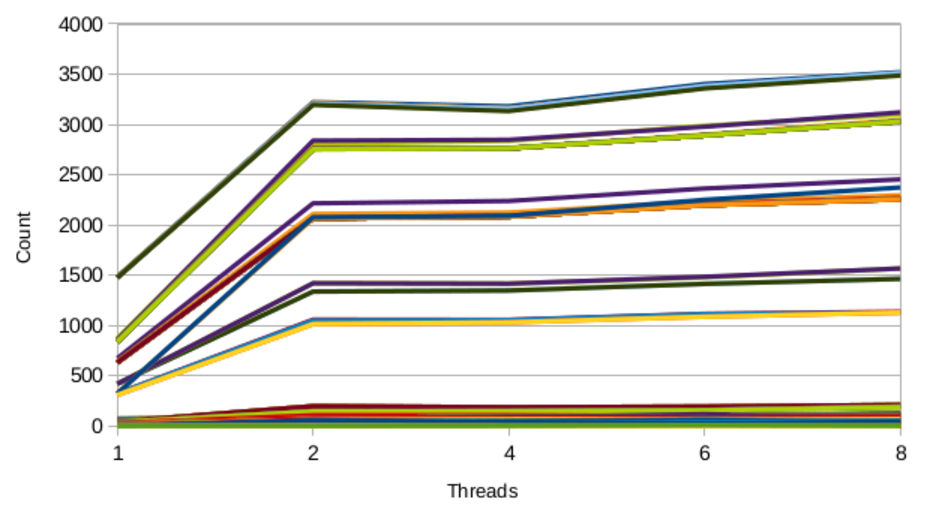
\includegraphics[width=0.4\textwidth]{images/cp2k-omp-inc-full.pdf}
\end{center}
\caption{Sampled reference counts to variables within OpenMP parallel regions}
\label{fig:openmp-refcount}
\end{figure}
